\documentclass{beamer}
\usepackage{amsfonts,amsmath,oldgerm}
\usetheme{sintef}

\newcommand{\testcolor}[1]{\colorbox{#1}{\textcolor{#1}{test}}~\texttt{#1}}

\usefonttheme[onlymath]{serif}

\titlebackground*{assets/background}

% adicionar o numero na lista final da apresentação
\setbeamertemplate{bibliography item}{\insertbiblabel}

\newcommand{\hrefcol}[2]{\textcolor{cyan}{\href{#1}{#2}}}

\title{Optimizers in deep learning}
\course{CPE 727 - Deep Learning}
\author{Ana Clara Loureiro Cruz \and Bruno \and Emre \and Felipe}
\IDnumber{%
  \href{mailto:anaclaralcruz@poli.ufrj.br}{anaclaralcruz@poli.ufrj.br}\\
  \href{mailto:anaclaralcruz@poli.ufrj.br}{anaclaralcruz@poli.ufrj.br}\\
  \href{mailto:anaclaralcruz@poli.ufrj.br}{anaclaralcruz@poli.ufrj.br}\\
  \href{mailto:anaclaralcruz@poli.ufrj.br}{anaclaralcruz@poli.ufrj.br}
}

\begin{document}
\maketitle

\section{Introduction}

\begin{frame}{Why Optimizers Matter}
\begin{itemize}
  \item \textbf{Hard landscapes:} non-convex, ill-conditioned; plateaus/saddles/sharp minima.
  \item \textbf{Speed vs.\ stability:} momentum, adaptivity, curvature cues.
  \item \textbf{Generalization:} optimizer choice influences minima flatness and test accuracy.
  \item \textbf{Scaling:} large batches + mixed precision $\Rightarrow$ LARS/LAMB trust ratios.
  \item \textbf{Anisotropy:} coordinate-wise steps (Adagrad/RMSProp/AdamW).
  \item \textbf{Decay:} AdamW’s decoupled weight decay matters.
  \item \textbf{Schedules:} warmup + cosine/one-cycle are often the real win.
\end{itemize}
\end{frame}

\begin{frame}{Intuition in Two Pictures}
\begin{columns}[T,onlytextwidth]
\begin{column}{0.48\textwidth}
\centering
\textbf{Sharp vs.\ Flat Minima}\\[0.3em]
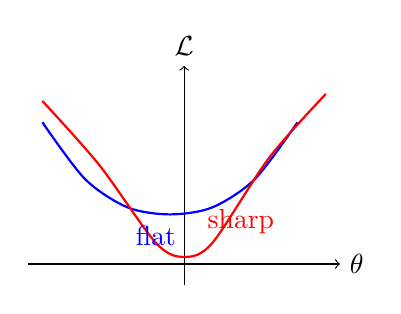
\begin{tikzpicture}[scale=0.9]
  \draw[->] (-2.2,0) -- (2.2,0) node[right] {$\theta$};
  \draw[->] (0,-0.3) -- (0,2.8) node[above] {$\mathcal{L}$};
  % flat well
  \draw[thick,blue] plot[smooth] coordinates {(-2,2) (-1.4,1.2) (-0.8,0.8) (-0.2,0.7) (0.4,0.8) (1.0,1.2) (1.6,2)};
  % sharp well
  \draw[thick,red] plot[smooth] coordinates {(-2,2.3) (-1.2,1.4) (-0.4,0.3) (0,0.1) (0.4,0.3) (1.2,1.5) (2,2.4)};
  \node[blue] at (-0.4,0.4) {flat};
  \node[red]  at (0.8,0.6)  {sharp};
\end{tikzpicture}

{\small SAM/SGD tend to favor flatter minima $\Rightarrow$ better test performance.}
\end{column}
\begin{column}{0.48\textwidth}
\centering
\textbf{Paths on an Anisotropic Bowl}\\[0.3em]
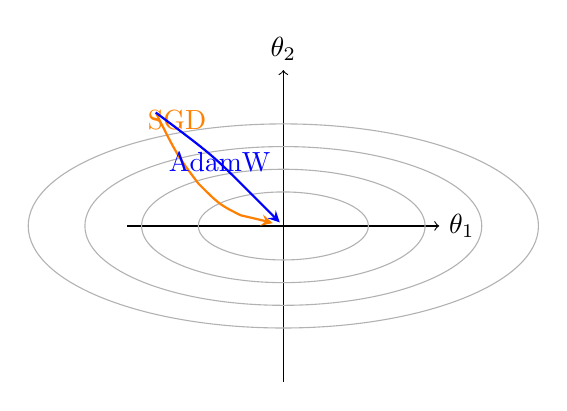
\begin{tikzpicture}[scale=0.9]
  % axes
  \draw[->] (-2.2,0) -- (2.2,0) node[right] {$\theta_1$};
  \draw[->] (0,-2.2) -- (0,2.2) node[above] {$\theta_2$};
  % contours (ellipses)
  \foreach \r in {0.6,1.0,1.4,1.8} {
    \draw[gray!60] (0,0) ellipse ({2*\r} and {0.8*\r});
  }
  % SGD path
  \draw[thick,orange,-stealth] (-1.8,1.6) .. controls (-1.5,1.0) .. (-1.2,0.6)
                                .. controls (-0.9,0.3) .. (-0.6,0.15) .. controls (-0.3,0.08) .. (-0.15,0.04);
  \node[orange] at (-1.5,1.5) {SGD};
  % AdamW path
  \draw[thick,blue,-stealth] (-1.8,1.6) .. controls (-1.0,1.0) .. (-0.5,0.5)
                             .. controls (-0.25,0.25) .. (-0.05,0.05);
  \node[blue] at (-0.9,0.9) {AdamW};
\end{tikzpicture}

{\small AdamW adapts steps per-coordinate; momentum smooths zig-zagging.}
\end{column}
\end{columns}
\end{frame}

\begin{frame}{Common notation}
Objective:  \min_\theta f(\theta)

Stochastic gradient at step t: g_t = \nabla_\theta f_t(\theta_t)

Base LR: \eta_t; small \varepsilon > 0 for numerical stability.
\end{frame}


\section{Plain First-Order}

\begin{frame}{SGD (baseline) \cite{gradientDescent}}
\[
  \theta_{t+1} = \theta_t - \eta_t\, g_t
\]
\begin{itemize}
  \item Sets the stage for momentum, adaptivity, and curvature.
  \item Sensitive to scale/conditioning; zig-zags in anisotropic valleys.
\end{itemize}
\textbf{Example:} \emph{SGD (vanilla)}
\end{frame}


\section{Momentum Variants}

\begin{frame}{Polyak \& Nesterov}
\textbf{Polyak Momentum (EMA of gradients):}
\[
  v_t = \beta\, v_{t-1} + (1-\beta)\, g_t,\qquad
  \theta_{t+1} = \theta_t - \eta_t\, v_t
\]
\textbf{Nesterov Momentum (look-ahead):}
\[
  \tilde{\theta}_t = \theta_t - \eta_t \beta v_{t-1},\quad
  v_t = \beta v_{t-1} + g(\tilde{\theta}_t),\quad
  \theta_{t+1} = \theta_t - \eta_t v_t
\]

\textbf{Example:} \emph{SGD + Momentum, Nesterov}
\end{frame}


\section{Adaptive First-Order}

\begin{frame}{Per-Coordinate Step Sizes}
\textbf{Adagrad (cumulative second moment):}
\[
  s_t = s_{t-1} + g_t \odot g_t,\qquad
  \theta_{t+1} = \theta_t - \frac{\eta}{\sqrt{s_t} + \varepsilon}\odot g_t
\]
\textbf{RMSProp (exponential second moment):}
\[
  s_t = \rho s_{t-1} + (1-\rho)\, g_t \odot g_t,\qquad
  \theta_{t+1} = \theta_t - \frac{\eta}{\sqrt{s_t} + \varepsilon}\odot g_t
\]
\end{frame}

\begin{frame}{Adam/AdamW and Friends}
\textbf{Adam (with bias correction):}
\[
  m_t=\beta_1 m_{t-1}+(1-\beta_1)g_t,\quad
  v_t=\beta_2 v_{t-1}+(1-\beta_2)g_t\odot g_t
\]
\[
  \hat m_t=\frac{m_t}{1-\beta_1^t},\quad
  \hat v_t=\frac{v_t}{1-\beta_2^t},\qquad
  \theta_{t+1}=\theta_t-\eta \frac{\hat m_t}{\sqrt{\hat v_t}+\varepsilon}
\]
\textbf{AdamW (decoupled weight decay):}
\[
  \theta_{t+1} = (1-\eta\lambda)\,\theta_t \;-\; \eta \frac{\hat m_t}{\sqrt{\hat v_t}+\varepsilon}
\]

\textbf{Examples:} \emph{Adagrad, RMSProp, Adam, AMSGrad, AdamW, RAdam, Adan, Lion}
\end{frame}


\section{Large-Batch / Layer-Wise Scaling}

\begin{frame}{LARS (Layer-wise Adaptive Rate Scaling)}
For layer $\ell$ with weights $\theta^{(\ell)}$ and gradient $g^{(\ell)}$:
\[
  r^{(\ell)} = \frac{\|\theta^{(\ell)}\|_2}{\|g^{(\ell)}\|_2 + \varepsilon},\qquad
  \Delta \theta^{(\ell)} = -\,\eta\,\phi\, r^{(\ell)}\, g^{(\ell)}
\]
\[
  \theta^{(\ell)}_{t+1} = \theta^{(\ell)}_t + \Delta \theta^{(\ell)} \quad (\text{often with momentum})
\]
\end{frame}

\begin{frame}{LAMB (Layer-wise Adaptive Moments)}
Combine Adam-like direction with a LARS-like trust ratio:
\[
  \Delta^{(\ell)} = \frac{\hat m^{(\ell)}}{\sqrt{\hat v^{(\ell)}}+\varepsilon}\;(+\;\lambda\,\theta^{(\ell)}\text{ if coupled})
\]
\[
  r^{(\ell)}=\frac{\|\theta^{(\ell)}\|_2}{\|\Delta^{(\ell)}\|_2+\varepsilon},\qquad
  \theta^{(\ell)}_{t+1}=\theta^{(\ell)}_t - \eta\, r^{(\ell)}\, \Delta^{(\ell)}
\]
\end{frame}


\section{Generalization-Oriented Wrappers}

\begin{frame}{Sharpness-Aware Minimization (SAM)}
\textbf{Minimax view:} $\displaystyle \min_\theta \max_{\|\epsilon\|\le \rho} f(\theta+\epsilon)$
\[
  \epsilon_t = \rho \frac{g_t}{\|g_t\|_2} \quad \Rightarrow \quad
  g_t^{\text{SAM}} = \nabla f(\theta_t+\epsilon_t), \quad
  \theta_{t+1} = \theta_t - \eta\,\text{BaseOpt}(g_t^{\text{SAM}})
\]
\end{frame}

\begin{frame}{Lookahead (Optimizer Wrapper)}
Maintain a slow weight copy $\phi$ and fast inner updates $\theta$:
\[
  \theta \leftarrow \text{BaseOptSteps}(\theta),\qquad
  \phi \leftarrow \phi + \alpha(\theta - \phi),\qquad
  \theta \leftarrow \phi
\]
\begin{itemize}
  \item Stabilizes training; often improves robustness with negligible overhead.
\end{itemize}
\textbf{Example:} \emph{SAM, Lookahead}
\end{frame}


\section{Curvature-Aware / Second-Order-ish}

\begin{frame}{L-BFGS and Friends}
\textbf{L-BFGS (quasi-Newton):} uses limited-memory Hessian inverse approximation $H_t$:
\[
  p_t = - H_t\, g_t,\qquad \theta_{t+1} = \theta_t + \eta_t\, p_t
\]
\textbf{AdaHessian (diagonal Hessian):}
\[
  h_t \approx \operatorname{diag}\!\big(\nabla^2 f(\theta_t)\big),\qquad
  \theta_{t+1} = \theta_t - \eta \frac{m_t}{\sqrt{h_t}+\varepsilon}
\]

\textbf{Examples:} \emph{L-BFGS, K-FAC, Shampoo, AdaHessian, Sophia}
\end{frame}

\section{Summary}

% ===== Slide 1: Baselines, Adaptive, Large-batch =====
\begin{frame}{Optimizer Summary (I): Baselines, Adaptive, Large-batch}
\scriptsize
\setlength{\tabcolsep}{3pt}
\renewcommand{\arraystretch}{1.25}
\begin{tabular}{p{2.8cm} p{4.3cm} p{4.5cm} p{3.5cm}}
\textbf{Method} & \textbf{Strengths / Behavior} & \textbf{Best Use Cases} & \textbf{Pitfalls \& Typical HPs} \\
\hline
\textbf{SGD + Nesterov} &
Low memory; strong generalization; stable with cosine schedule; Nesterov gives look-ahead acceleration &
CNNs/vision, medium batches; when you can tune LR/schedule & 
Can be slow on ill-conditioned problems; $\eta\!\in[0.1,0.01]$ (scale w/ batch), momentum $0.9$, cosine + warmup \\

\textbf{Adagrad} &
Per-coordinate steps; great on sparse features; no LR tuning once set &
Sparse NLP/recsys embeddings; convex-ish problems &
Learning rate “dies” (accumulator grows); $\eta\!\in[0.05,0.01]$, $\varepsilon\!\sim\!10^{-10}$ \\

\textbf{RMSProp} &
Controls step via EMA of squared grads; steadier than Adagrad &
RNN-ish/online settings; when gradient scales drift &
Sensitive to $\rho$; defaults: $\eta\!\in[10^{-3},10^{-4}],\ \rho\!=\!0.9,\ \varepsilon\!\sim\!10^{-8}$ \\

\textbf{AdamW} &
Fast convergence; bias correction; \emph{decoupled} weight decay improves generalization vs L2 &
Transformers/ViTs/LLMs; mixed precision; general default &
May overfit vs SGD on some vision tasks; $\eta\!\in[3\!\times\!10^{-4},10^{-4}],\ \beta=(0.9,0.999),\ \text{wd}\!=\!0.01$ \\

\textbf{AMSGrad / RAdam} &
AMSGrad: non-increasing second moment; RAdam: rectifies early variance &
When Adam is unstable early or drifts &
Slightly slower than AdamW sometimes; use AdamW-like HPs \\

\textbf{Lion} &
Momentum on \emph{sign}; memory-light; competitive on vision/NLP &
Resource-constrained training; quick baselines &
Tuning can differ from AdamW; $\eta$ often higher; $\beta\!\approx\!(0.9,0.99)$ \\

\textbf{Adan} &
Uses gradient differences + Nesterov-style look-ahead; strong empirically on vision &
Vision with medium/large models; noisy grads &
More knobs; start from authors’ defaults \\

\textbf{LARS} &
Layer-wise trust ratio keeps per-layer steps well-scaled &
Very large-batch CNNs on ImageNet (8k–32k+ batch) &
Needs warmup; trust-ratio clipping; pair with momentum/cosine \\

\textbf{LAMB} &
Adam-direction + trust ratio (LARS-like); scales BERT/ViTs to huge batches &
Huge-batch transformers; multi-node training &
Tune weight decay + warmup; trust ratio can over-scale some layers \\
\end{tabular}
\end{frame}

% ===== Slide 2: Wrappers, Curvature-aware, Schedules =====
\begin{frame}{Optimizer Summary (II): Generalization, Curvature, Schedules}
\scriptsize
\setlength{\tabcolsep}{3pt}
\renewcommand{\arraystretch}{1.25}
\begin{tabular}{p{2.8cm} p{4.3cm} p{4.5cm} p{3.5cm}}
\textbf{Method} & \textbf{Strengths / Behavior} & \textbf{Best Use Cases} & \textbf{Pitfalls \& Typical HPs} \\
\hline
\textbf{SAM (wrapper)} &
Minimax: avoids sharp minima; often boosts test accuracy &
Vision/ViTs where generalization matters; pair with SGD/AdamW &
Extra forward/backward; radius $\rho\!\in\![0.05,0.2]$; keep weight decay decoupled \\

\textbf{Lookahead (wrapper)} &
Slow–fast weights; stabilizes training; cheap &
Add on top of AdamW/SGD for robustness &
Sync period/alpha add knobs; small but consistent gains \\

\textbf{L-BFGS (quasi-Newton)} &
Fast on smooth/convex-ish, small problems; strong steps &
Small models, fine-tuning last layers; classic ML &
Not mini-batch-friendly; line search overhead; memory for history \\

\textbf{K-FAC} &
Kronecker-factored curvature; fewer steps to good loss &
Deep nets when you can afford extra compute; large-scale setups &
Complex to implement/distribute; extra memory/compute \\

\textbf{Shampoo} &
Factored preconditioning per tensor; strong practical results &
Large models at scale (when infra supports it) &
Higher memory; tuning preconditioner update periods \\

\textbf{AdaHessian} &
Diagonal Hessian via stochastic probes; 2nd-order flavor w/ modest cost &
When AdamW plateaus and curvature helps &
Noisy Hessian diag; tune probe count; $\eta$ similar to AdamW \\

\textbf{Sophia} &
Light-weight curvature proxy; good for LLM pretraining &
Large language models; budget-aware curvature &
Proxy quality/task-dependent; follow paper defaults \\

\textbf{Schedules (orthogonal)} &
Cosine/one-cycle + warmup often \emph{bigger} gains than swapping optimizers &
Always apply: large-batch, mixed precision, transformers/CNNs &
Choose warmup length (1–5\% of steps); use gradient clipping and EMA of weights for eval \\
\end{tabular}
\end{frame}


\section{References} 
\begin{frame}[allowframebreaks]
        \frametitle{Referências Bibliográficas} 
        \bibliographystyle{ieeetr}
        \bibliography{presentation_bib.bib}
\end{frame}


\backmatter
\end{document}
